\chapter[Introdução]{Introdução}
%\addcontentsline{toc}{chapter}{Introdução}

\section{Contextualização}
	
	O nascimento da robótica se deu no contexto industrial, no qual ferramentas autônomas foram desenvolvidas para executar atividades de forma repetitiva e incansável, maximizando a qualidade dos produtos e minimizando o custo e tempo para produção dos mesmos \cite{roboticaIndustrial}. Segundo \cite{roboticaIndustrial}, a palavra robô é derivada da palavra \textit{robota}, de origem eslava, que significa \textit{trabalho forçado}, ou seja, robôs podem ser considerados ferramentas incansáveis que apoiam o trabalho humano. 

	Segundo \cite{localizacaoEMapeamentoPaulo}, a autonomia de um robô é condicionada pela sua capacidade de perceber o ambiente de navegação, interagindo com o meio e realizando tarefas com o mínimo de precisão. Este mínimo, de acordo com \cite{localizacaoEMapeamentoPaulo}, seria a navegação sem colisão em obstáculos. 

	Para que robôs sejam capazes de navegar em um ambiente desconhecido sem que haja colisão em objetos e obstáculos, os mesmos necessitam de informações sobre este ambiente. Estas informações são adquiridas utilizando sensores. Como foi apresentado por \cite{interacaoRoboAmbiente}, no livro de Robótica Industrial, os sensores possuem o dever de fornecer informações ao sistema de controle do robô sobre distâncias de objetos, posição do robô, contato do robô com objetos, força exercida sobre objetos, cor e textura dos objetos, entre outras.

	Além de obter dados sobre o ambiente, o robô precisa se auto-localizar para processar as informações obtidas e traçar rotas sem colisões até o ponto de destino. Para isso, foram desenvolvidas muitas formas de auto-localização, algumas delas são citadas por \cite{roboBulldozerIV}, como:

	\begin{itemize}
		\item \textbf{Utilização de Mapas}: O robô conhece o mapa onde realizará a navegação à priori, conhecendo os obstáculos e os caminhos possíveis. Possuindo essas informações, o robô irá traçar as rotas mais eficientes para chegar em seu objetivo.

		\item \textbf{Localização Relativa em Grupos}: Esta técnica utiliza a navegação simultânea de muitos robôs, cada robô sabe a posição relativa dos outros robôs, podendo calcular sua posição relativa.

		\item \textbf{Utilização de Pontos de Referência}: Conhecendo pontos de referência que estão distribuídos pelo mapa de navegação, o robô consegue calcular sua posição através da técnica de triangulação.

		\item \textbf{Localização Absoluta com GPS}: A partir desta técnica, é fácil obter a posição absoluta do robô em relação à terra. O grande problema desta técnica é a margem de erro presente no sistema de GPS, inviável para navegações internas.

		\item \textbf{Utilização de Bússolas}: É uma técnica interessante para reconhecimento da orientação do robô, o que facilita muito na navegação do mesmo. Entretando, as Bússolaslas são muito frágeis a interferências externas, como por exemplo, a proximidade de materiais ferro-magnéticos ou as fugas magnéticas dos motores presentes no próprio robô.

		\item \textbf{Odometria}: Consiste na medição da distância relativa percorrida pelo robô, utilizando sensores presentes nas rodas do mesmo. Necessita do conhecimento do ponto de origem.
		 
	\end{itemize}

	As formas apresentadas anteriormente, para se trabalhar com auto-localização, possuem características únicas que as adequam para diferentes contextos de navegação. Por exemplo, segundo \cite{roboBulldozerIV}, a Utilização de Mapas é uma técnica bastante útil quando se está trabalhando com um ambiente conhecido e estático, porém, em ambientes mutáveis e não conhecidos, essa estratégia se torna um problema. A Localização Relativa em Grupos é a técnica adequada quando a navegação envolve muitos robôs, a qual não necessita de conhecimento prévio do mapa. A Utilização de Pontos de Referência é uma técnica comumente utilizada, é útil quando não se conhece o ambiente de navegação. Entretanto, os pontos de referência, nesse caso, precisam ser conhecidos. 

	Quando se têm ambientes abertos e amplos, a técnica de Localização Absoluta com GPS é a mais utilizada. Entretanto, sua margem de erro torna a navegação em ambientes pequenos ou fechados inviável, como apresenta \cite{roboBulldozerIV}. A Navegação com utilização de Bússulas garante um apoio muito útil para orientação do robô. Contudo, essa técnica gera problemas relacionados a interferências externas, como materiais eletromagnéticos próximos à bússula \cite{roboBulldozerIV}.
	
	A técnica de Odometria é muito utilizada em navegações curtas, em ambientes com o piso regular e plano. Entretando, segundo \cite{roboBulldozerIV}, esta técnica se caracteriza pela adição de erros a cada centímetro percorrido, por meio de derrapagens e falhas no giro das rodas. 

	Desse modo, é fácil perceber que cada técnica possui características que se adaptam melhor para diferentes situações. Ao longo deste trabalho, o principal foco de interesse é a navegabilidade de robôs simples e baratos, como os Kit Lego Mindstorms\footnote{mindstorms.lego.com}. Tais kits possuem poucas opções de sensores e características bem limitadas \cite{drawLegoRobot}. Os sensores do kit que serão utilizados neste trabalho são: \textit{Sensor de proximidade, sensor RGB, sensor de contato e sensor odométrico}.

\section{Problema de Pesquisa}

	Todas as técnicas de auto-localização apresentadas na seção anterior já foram testadas, comparadas e refatoradas em diferentes contextos, desde a navegação marítima até questões relacionadas à tecnologia aeroespacial \cite{localizacaoEMapeamentoPaulo}. Porém, sabe-se que, nestes contextos, o \textit{hardware} utilizado para navegação era de alta tecnologia, possuindo processadores de altíssimo desempenho e sensores bem precisos.

	Já em um contexto educacional, a infraestrutura disponível nem sempre engloba os critérios necessários para aplicação das técnicas de auto-localização. Um exemplo disso é a utilização, por \cite{localizacaoEMapeamentoPaulo}, de uma câmera omnidirecional para obter informações sobre o ambiente.

	Desse modo, vê-se a necessidade da adaptação de técnicas de auto-localização para o contexto da Robótica Educacional, utilizando os kits de robótica \textit{Mindstorms} da LEGO. Nesses kits, a capacidade de processamento e a precisão dos sensores e dos atuadores são limitadas. A intenção é tomar como base a técnica de mapeamento do ambiente e auto-localização simultâneos (conhecida como problema de SLAM - \textit{Simultaneous Location and Mapping}) \cite{slamProblem}.

	A questão de pesquisa que será discutida durante este trabalho é \textit{"Como tratar o problema de SLAM no contexto de robôs simples?"}.

\section{Justificativa}

	A utilização da Robótica como uma forma de ensinar programação em escolas e faculdades, conhecida como Robótica Educacional \cite{roboticaEducacionalAulasMatematica}, traz alguns benefícios para o aluno. Conforme colocado pelos autores \cite{teachingWithRoboticKit}, \cite{roboticEducationBasedLego}, \cite{roboticaEducacionalAulasMatematica} e \cite{evaluationRoboticEducationScale}, alguns desses benefícios são: 
	\begin{itemize}
		\item Maior interesse pelos conteúdos estudados em aula;
		\item capacidade de trabalhar em grupo;
		\item aplicação prática do conhecimento teórico;
		\item multidisciplinaridade.
	\end{itemize}
	 
	 A Universidade de Brasília utiliza esta abordagem de ensino/aprendizagem durante a disciplina de Introdução à Robótica Educacional, ministrada em 2016, pelo professor Dr. Maurício Serrano. A disciplina utiliza os Kits de robótica Mindstorms, da Lego, para desenvolvimento de soluções dos problemas presentes em um tapete de missões. A organização da disciplina se inspira nos campeonatos de robótica, como o \textit{ciber-rato} \cite{ciber-rato} ou \textit{micro-rato} \cite{roboBulldozerIV}. Neste tipo de campeonato, a navegação é o quesito mais importante \cite{ciber-rato}, a qual deve possuir a menor margem de erro para solucionar as missões.

	As missões utilizadas durante a disciplina da UnB são referentes a problemas recorrentes no contexto da robótica mundial. A solução dos problemas é uma adaptação das técnicas existentes para o contexto limitado da disciplina, onde são utilizadas apenas ferramentas presentes no kit \textit{Mindstorms} da Lego. Esta adaptação exige um conhecimento específico sobre a técnica, para que o estudante possa identificar características relevantes e adaptá-las de acordo com o \textit{hardware} disponível.

	A disciplina já influenciou dois estudantes de Engenharia de Software a se aprofundarem no contexto da robótica e robótica educacional, gerando dois trabalhos de conclusão de curso, \cite{tccRodrigo}, que desenvolveu um \textit{framework} de definição de trajetórias para robôs móveis, e \cite{tccCarol}, que desenvolveu um algorítmo para tomada de decisões estratégicas em robótica educacional. O trabalho atual vem para complementar os trabalhos realizados pelos dois alunos.


	\section{Objetivos}

	\subsection{Objetivo Geral} % (fold)
	\label{sub:objetivos_gerais}
	
		Adaptar técnicas de resolução do problema de SLAM para o contexto de robôs simples, utilizando os kits de robótica \textit{Mindstorms} da Lego, em um primeiro momento.

	% subsection objetivos_gerais (end)

	\subsection{Objetivos Específicos} % (fold)
	\label{sub:objetivos_específicos}
		 
	\begin{itemize}
		\item Solucionar o problema de SLAM;
		\item Propor adaptação pro contexto de robôs simples, na robótica educacional;
		\item Implementar adaptação.
	\end{itemize}
	
	% subsection objetivos_específicos (end)

	\section[Metodologia]{Metodologia}

Este trabalho segue uma metodologia de pesquisa exploratória e com uma abordagem qualitativa, onde são selecionadas, comparadas e analisadas técnicas de resolução do problema de SLAM. De acordo com \cite{metodologiaCientifica}, a pesquisa exploratória tem como objetivo ampliar os conhecimentos do pesquisador sobre o tema. O uso da pesquisa exploratória, neste trabalho, se dá pela necessidade do conhecimento sobre as técnicas de resolução do problema de SLAM, com o intuito de realizar adaptações das mesmas para o contexto de robôs simples. Já a abordagem qualitativa, tem como objetivo entender o funcionamento e as técnicas existentes, para buscar uma forma de adaptação para um contexto simplificado, não se importando com dados quantificáveis.

Com o objetivo de identificar o máximo de técnicas possíveis, com os mais diferentes tipos de \textit{hardwares}, será realizada uma pesquisa bibliográfica sobre os temas \textit{Auto-localização na Robótica, o Problema de SLAM e as características dos robôs simples presentes na Robótica Educacional}. As principais fontes de dados em estudo são as bases da CAPES, IEEE e Scopus.

A primeira fase deste trabalho é focada em estabelecer pilares teóricos que sustentem um projeto de adaptação de técnicas durante a segunda fase. Esta primeira fase pode ser sub-dividida em três atividades: \textit{Realizar Pesquisa Bibliográfica}, \textit{selecionar Técnicas} e \textit{Propor Adaptações}. As mesmas estão distribuídas de acordo com o cronograma disposto na tabela \ref{tab:cronograma}.

\begin{table}[http]
	\centering
	\caption{Cronograma TCC 1}
	\label{tab:cronograma}
	\begin{tabular}{ccccc}
		\hline
		\multicolumn{1}{|c|}{\textbf{Cronograma}}             & \multicolumn{1}{c|}{\textbf{Março}} & \multicolumn{1}{c|}{\textbf{Abril}} & \multicolumn{1}{c|}{\textbf{Maio}} & \multicolumn{1}{c|}{\textbf{Junho}} \\ \hline
		\multicolumn{1}{|c|}{Realizar Pesquisa Bibliográfica} & \multicolumn{1}{c|}{X}              & \multicolumn{1}{c|}{X}              & \multicolumn{1}{c|}{X}             & \multicolumn{1}{c|}{X}              \\ \hline
		\multicolumn{1}{|c|}{Selecionar técnicas}             & \multicolumn{1}{c|}{}               & \multicolumn{1}{c|}{X}              & \multicolumn{1}{c|}{X}             & \multicolumn{1}{c|}{}               \\ \hline
		\multicolumn{1}{|c|}{Propor adaptação}                & \multicolumn{1}{c|}{}               & \multicolumn{1}{c|}{}               & \multicolumn{1}{c|}{X}             & \multicolumn{1}{c|}{X}              \\ \hline
		\multicolumn{1}{l}{}                                  & \multicolumn{1}{l}{}                & \multicolumn{1}{l}{}                & \multicolumn{1}{l}{}               & \multicolumn{1}{l}{}                \\
		\multicolumn{1}{l}{}                                  & \multicolumn{1}{l}{}                & \multicolumn{1}{l}{}                & \multicolumn{1}{l}{}               & \multicolumn{1}{l}{}                \\
		\multicolumn{1}{l}{}                                  & \multicolumn{1}{l}{}                & \multicolumn{1}{l}{}                & \multicolumn{1}{l}{}               & \multicolumn{1}{l}{}               
	\end{tabular}
\end{table}

Com o objetivo de definir e acompanhar o processo de desenvolvimento da primeira etapa do trabalho de conclusão de curso, foi modelado um processo metodológico, o qual se encontra na figura \ref{img:processo}.

\begin{figure}[H]
	\centering
	\caption{Processo Metodológico}
	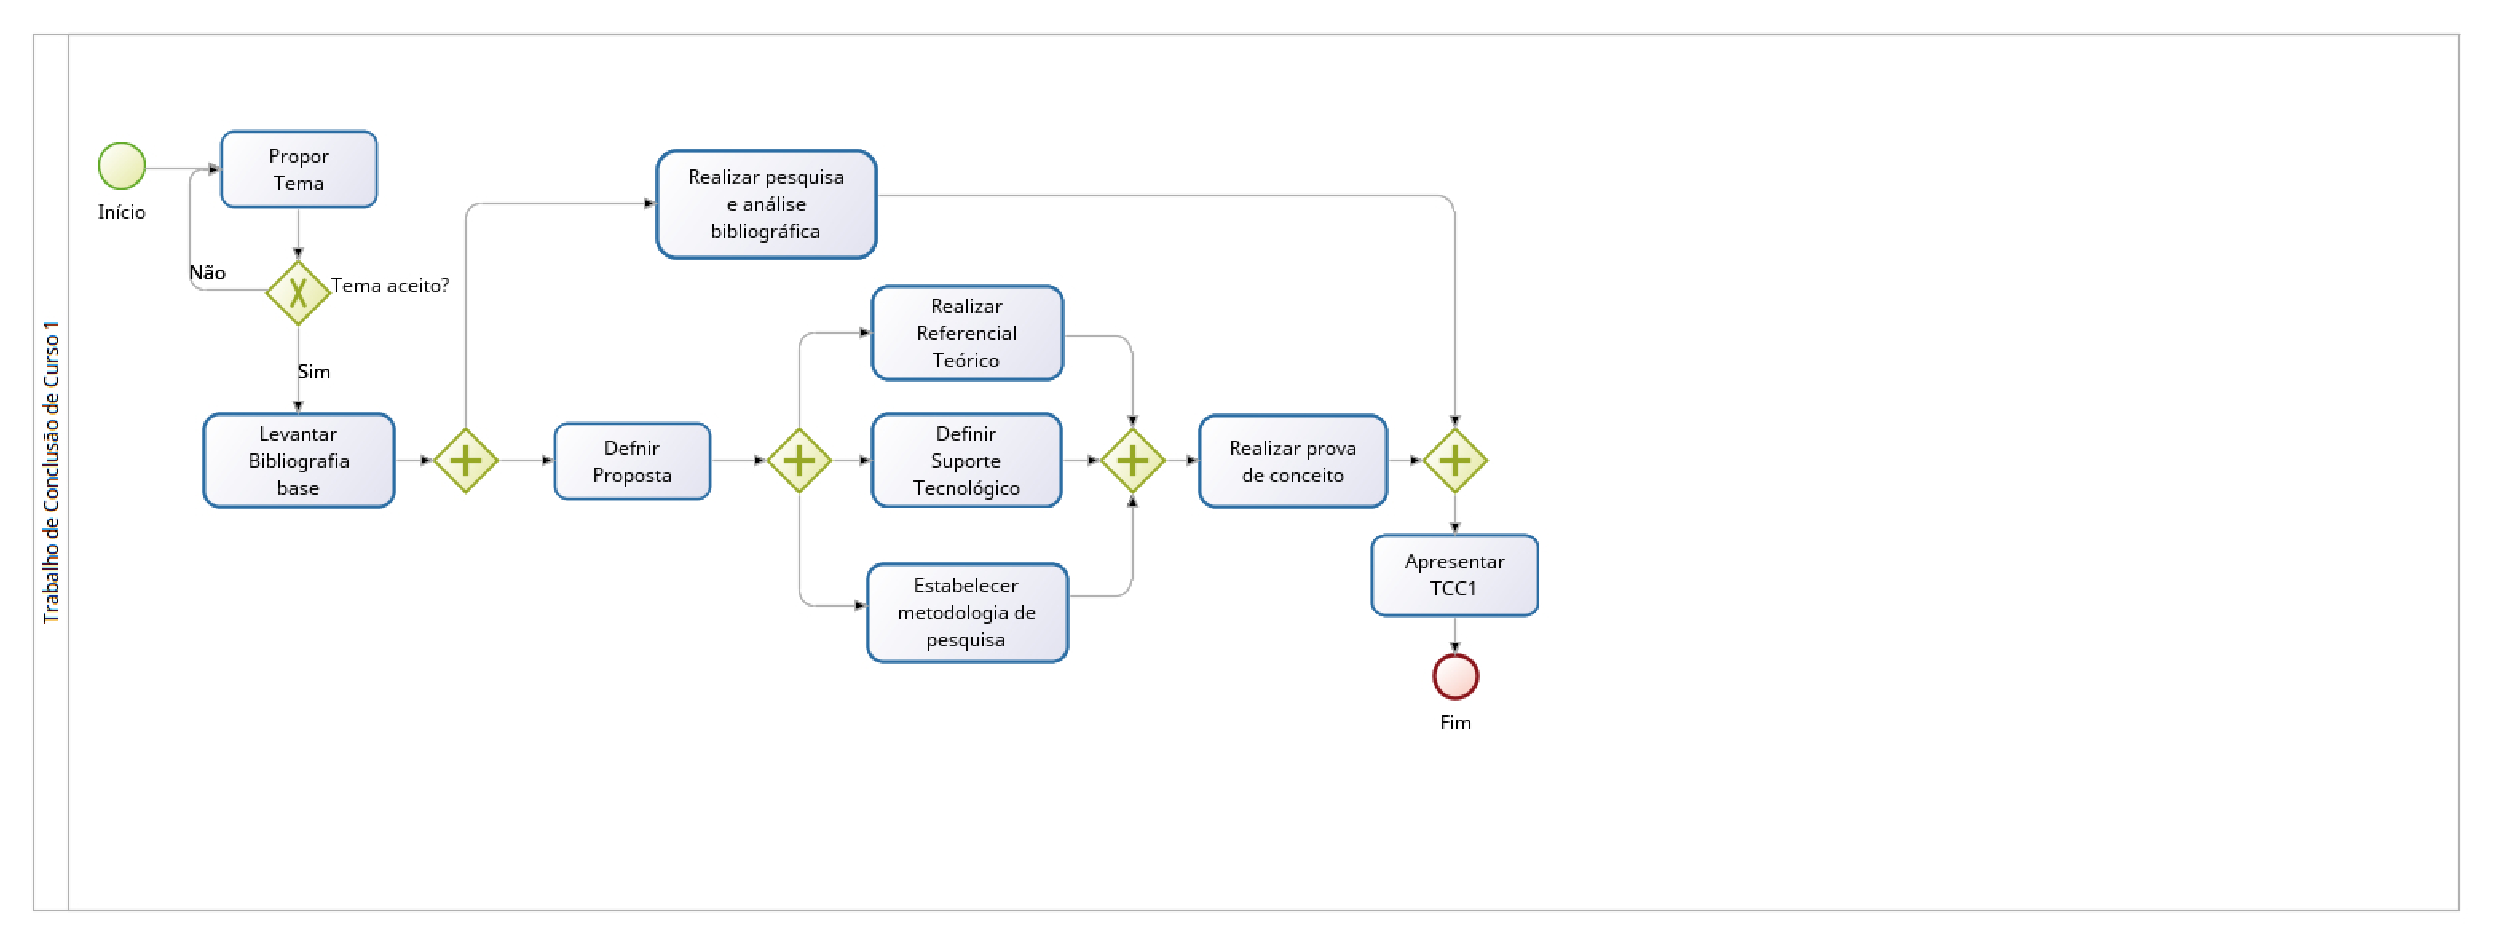
\includegraphics[scale=0.6]{figuras/processo.eps}
	\label{img:processo}
\end{figure}

Para colaborar com o entendimento do processo, as atividades e condições presentes no mesmo são descritas a seguir.

\begin{itemize}
	\item 
\end{itemize}
%Quanto aos procedimentos de desenvolvimento, durante a fase de adaptação de técnicas de resolução do problema de SLAM, a metodologia seguida será baseada no \textit{Scrum}, utilizando sprints de 2 semanas. O desenvolvimento se dará com base em provas de conceito que buscarão sustentar a viabilidade das adaptações propostas.
